%% bare_jrnl.tex
%% V1.4b
%% 2015/08/26
%% by Michael Shell
%% see http://www.michaelshell.org/
%% for current contact information.
%%
%% This is a skeleton file demonstrating the use of IEEEtran.cls
%% (requires IEEEtran.cls version 1.8b or later) with an IEEE
%% journal paper.
%%
%% Support sites:
%% http://www.michaelshell.org/tex/ieeetran/
%% http://www.ctan.org/pkg/ieeetran
%% and
%% http://www.ieee.org/

%%*************************************************************************
%% Legal Notice:
%% This code is offered as-is without any warranty either expressed or
%% implied; without even the implied warranty of MERCHANTABILITY or
%% FITNESS FOR A PARTICULAR PURPOSE! 
%% User assumes all risk.
%% In no event shall the IEEE or any contributor to this code be liable for
%% any damages or losses, including, but not limited to, incidental,
%% consequential, or any other damages, resulting from the use or misuse
%% of any information contained here.
%%
%% All comments are the opinions of their respective authors and are not
%% necessarily endorsed by the IEEE.
%%
%% This work is distributed under the LaTeX Project Public License (LPPL)
%% ( http://www.latex-project.org/ ) version 1.3, and may be freely used,
%% distributed and modified. A copy of the LPPL, version 1.3, is included
%% in the base LaTeX documentation of all distributions of LaTeX released
%% 2003/12/01 or later.
%% Retain all contribution notices and credits.
%% ** Modified files should be clearly indicated as such, including  **
%% ** renaming them and changing author support contact information. **
%%*************************************************************************


% *** Authors should verify (and, if needed, correct) their LaTeX system  ***
% *** with the testflow diagnostic prior to trusting their LaTeX platform ***
% *** with production work. The IEEE's font choices and paper sizes can   ***
% *** trigger bugs that do not appear when using other class files.       ***                          ***
% The testflow support page is at:
% http://www.michaelshell.org/tex/testflow/


% Please refer to your journal's instructions for other
% options that should be set.
\documentclass[journal,onecolumn]{IEEEtran}
%
% If IEEEtran.cls has not been installed into the LaTeX system files,
% manually specify the path to it like:
% \documentclass[journal]{../sty/IEEEtran}





% Some very useful LaTeX packages include:
% (uncomment the ones you want to load)


% *** MISC UTILITY PACKAGES ***
%
%\usepackage{ifpdf}
% Heiko Oberdiek's ifpdf.sty is very useful if you need conditional
% compilation based on whether the output is pdf or dvi.
% usage:
% \ifpdf
%   % pdf code
% \else
%   % dvi code
% \fi
% The latest version of ifpdf.sty can be obtained from:
% http://www.ctan.org/pkg/ifpdf
% Also, note that IEEEtran.cls V1.7 and later provides a builtin
% \ifCLASSINFOpdf conditional that works the same way.
% When switching from latex to pdflatex and vice-versa, the compiler may
% have to be run twice to clear warning/error messages.






% *** CITATION PACKAGES ***
%
%\usepackage{cite}
% cite.sty was written by Donald Arseneau
% V1.6 and later of IEEEtran pre-defines the format of the cite.sty package
% \cite{} output to follow that of the IEEE. Loading the cite package will
% result in citation numbers being automatically sorted and properly
% "compressed/ranged". e.g., [1], [9], [2], [7], [5], [6] without using
% cite.sty will become [1], [2], [5]--[7], [9] using cite.sty. cite.sty's
% \cite will automatically add leading space, if needed. Use cite.sty's
% noadjust option (cite.sty V3.8 and later) if you want to turn this off
% such as if a citation ever needs to be enclosed in parenthesis.
% cite.sty is already installed on most LaTeX systems. Be sure and use
% version 5.0 (2009-03-20) and later if using hyperref.sty.
% The latest version can be obtained at:
% http://www.ctan.org/pkg/cite
% The documentation is contained in the cite.sty file itself.






% *** GRAPHICS RELATED PACKAGES ***
%
\ifCLASSINFOpdf
  % \usepackage[pdftex]{graphicx}
  % declare the path(s) where your graphic files are
  % \graphicspath{{../pdf/}{../jpeg/}}
  % and their extensions so you won't have to specify these with
  % every instance of \includegraphics
  % \DeclareGraphicsExtensions{.pdf,.jpeg,.png}
\else
  % or other class option (dvipsone, dvipdf, if not using dvips). graphicx
  % will default to the driver specified in the system graphics.cfg if no
  % driver is specified.
  % \usepackage[dvips]{graphicx}
  % declare the path(s) where your graphic files are
  % \graphicspath{{../eps/}}
  % and their extensions so you won't have to specify these with
  % every instance of \includegraphics
  % \DeclareGraphicsExtensions{.eps}
\fi
% graphicx was written by David Carlisle and Sebastian Rahtz. It is
% required if you want graphics, photos, etc. graphicx.sty is already
% installed on most LaTeX systems. The latest version and documentation
% can be obtained at: 
% http://www.ctan.org/pkg/graphicx
% Another good source of documentation is "Using Imported Graphics in
% LaTeX2e" by Keith Reckdahl which can be found at:
% http://www.ctan.org/pkg/epslatex
%
% latex, and pdflatex in dvi mode, support graphics in encapsulated
% postscript (.eps) format. pdflatex in pdf mode supports graphics
% in .pdf, .jpeg, .png and .mps (metapost) formats. Users should ensure
% that all non-photo figures use a vector format (.eps, .pdf, .mps) and
% not a bitmapped formats (.jpeg, .png). The IEEE frowns on bitmapped formats
% which can result in "jaggedy"/blurry rendering of lines and letters as
% well as large increases in file sizes.
%
% You can find documentation about the pdfTeX application at:
% http://www.tug.org/applications/pdftex

\usepackage{graphicx}
\usepackage{placeins}
\usepackage{mathtools}
\usepackage{listings}
\usepackage{threeparttable}
\graphicspath{ {./img/} }



% *** MATH PACKAGES ***
%
%\usepackage{amsmath}
% A popular package from the American Mathematical Society that provides
% many useful and powerful commands for dealing with mathematics.
%
% Note that the amsmath package sets \interdisplaylinepenalty to 10000
% thus preventing page breaks from occurring within multiline equations. Use:
%\interdisplaylinepenalty=2500
% after loading amsmath to restore such page breaks as IEEEtran.cls normally
% does. amsmath.sty is already installed on most LaTeX systems. The latest
% version and documentation can be obtained at:
% http://www.ctan.org/pkg/amsmath





% *** SPECIALIZED LIST PACKAGES ***
%
%\usepackage{algorithmic}
% algorithmic.sty was written by Peter Williams and Rogerio Brito.
% This package provides an algorithmic environment fo describing algorithms.
% You can use the algorithmic environment in-text or within a figure
% environment to provide for a floating algorithm. Do NOT use the algorithm
% floating environment provided by algorithm.sty (by the same authors) or
% algorithm2e.sty (by Christophe Fiorio) as the IEEE does not use dedicated
% algorithm float types and packages that provide these will not provide
% correct IEEE style captions. The latest version and documentation of
% algorithmic.sty can be obtained at:
% http://www.ctan.org/pkg/algorithms
% Also of interest may be the (relatively newer and more customizable)
% algorithmicx.sty package by Szasz Janos:
% http://www.ctan.org/pkg/algorithmicx




% *** ALIGNMENT PACKAGES ***
%
%\usepackage{array}
% Frank Mittelbach's and David Carlisle's array.sty patches and improves
% the standard LaTeX2e array and tabular environments to provide better
% appearance and additional user controls. As the default LaTeX2e table
% generation code is lacking to the point of almost being broken with
% respect to the quality of the end results, all users are strongly
% advised to use an enhanced (at the very least that provided by array.sty)
% set of table tools. array.sty is already installed on most systems. The
% latest version and documentation can be obtained at:
% http://www.ctan.org/pkg/array


% IEEEtran contains the IEEEeqnarray family of commands that can be used to
% generate multiline equations as well as matrices, tables, etc., of high
% quality.




% *** SUBFIGURE PACKAGES ***
%\ifCLASSOPTIONcompsoc
%  \usepackage[caption=false,font=normalsize,labelfont=sf,textfont=sf]{subfig}
%\else
%  \usepackage[caption=false,font=footnotesize]{subfig}
%\fi
% subfig.sty, written by Steven Douglas Cochran, is the modern replacement
% for subfigure.sty, the latter of which is no longer maintained and is
% incompatible with some LaTeX packages including fixltx2e. However,
% subfig.sty requires and automatically loads Axel Sommerfeldt's caption.sty
% which will override IEEEtran.cls' handling of captions and this will result
% in non-IEEE style figure/table captions. To prevent this problem, be sure
% and invoke subfig.sty's "caption=false" package option (available since
% subfig.sty version 1.3, 2005/06/28) as this is will preserve IEEEtran.cls
% handling of captions.
% Note that the Computer Society format requires a larger sans serif font
% than the serif footnote size font used in traditional IEEE formatting
% and thus the need to invoke different subfig.sty package options depending
% on whether compsoc mode has been enabled.
%
% The latest version and documentation of subfig.sty can be obtained at:
% http://www.ctan.org/pkg/subfig




% *** FLOAT PACKAGES ***
%
%\usepackage{fixltx2e}
% fixltx2e, the successor to the earlier fix2col.sty, was written by
% Frank Mittelbach and David Carlisle. This package corrects a few problems
% in the LaTeX2e kernel, the most notable of which is that in current
% LaTeX2e releases, the ordering of single and double column floats is not
% guaranteed to be preserved. Thus, an unpatched LaTeX2e can allow a
% single column figure to be placed prior to an earlier double column
% figure.
% Be aware that LaTeX2e kernels dated 2015 and later have fixltx2e.sty's
% corrections already built into the system in which case a warning will
% be issued if an attempt is made to load fixltx2e.sty as it is no longer
% needed.
% The latest version and documentation can be found at:
% http://www.ctan.org/pkg/fixltx2e


%\usepackage{stfloats}
% stfloats.sty was written by Sigitas Tolusis. This package gives LaTeX2e
% the ability to do double column floats at the bottom of the page as well
% as the top. (e.g., "\begin{figure*}[!b]" is not normally possible in
% LaTeX2e). It also provides a command:
%\fnbelowfloat
% to enable the placement of footnotes below bottom floats (the standard
% LaTeX2e kernel puts them above bottom floats). This is an invasive package
% which rewrites many portions of the LaTeX2e float routines. It may not work
% with other packages that modify the LaTeX2e float routines. The latest
% version and documentation can be obtained at:
% http://www.ctan.org/pkg/stfloats
% Do not use the stfloats baselinefloat ability as the IEEE does not allow
% \baselineskip to stretch. Authors submitting work to the IEEE should note
% that the IEEE rarely uses double column equations and that authors should try
% to avoid such use. Do not be tempted to use the cuted.sty or midfloat.sty
% packages (also by Sigitas Tolusis) as the IEEE does not format its papers in
% such ways.
% Do not attempt to use stfloats with fixltx2e as they are incompatible.
% Instead, use Morten Hogholm'a dblfloatfix which combines the features
% of both fixltx2e and stfloats:
%
% \usepackage{dblfloatfix}
% The latest version can be found at:
% http://www.ctan.org/pkg/dblfloatfix




%\ifCLASSOPTIONcaptionsoff
%  \usepackage[nomarkers]{endfloat}
% \let\MYoriglatexcaption\caption
% \renewcommand{\caption}[2][\relax]{\MYoriglatexcaption[#2]{#2}}
%\fi
% endfloat.sty was written by James Darrell McCauley, Jeff Goldberg and 
% Axel Sommerfeldt. This package may be useful when used in conjunction with 
% IEEEtran.cls'  captionsoff option. Some IEEE journals/societies require that
% submissions have lists of figures/tables at the end of the paper and that
% figures/tables without any captions are placed on a page by themselves at
% the end of the document. If needed, the draftcls IEEEtran class option or
% \CLASSINPUTbaselinestretch interface can be used to increase the line
% spacing as well. Be sure and use the nomarkers option of endfloat to
% prevent endfloat from "marking" where the figures would have been placed
% in the text. The two hack lines of code above are a slight modification of
% that suggested by in the endfloat docs (section 8.4.1) to ensure that
% the full captions always appear in the list of figures/tables - even if
% the user used the short optional argument of \caption[]{}.
% IEEE papers do not typically make use of \caption[]'s optional argument,
% so this should not be an issue. A similar trick can be used to disable
% captions of packages such as subfig.sty that lack options to turn off
% the subcaptions:
% For subfig.sty:
% \let\MYorigsubfloat\subfloat
% \renewcommand{\subfloat}[2][\relax]{\MYorigsubfloat[]{#2}}
% However, the above trick will not work if both optional arguments of
% the \subfloat command are used. Furthermore, there needs to be a
% description of each subfigure *somewhere* and endfloat does not add
% subfigure captions to its list of figures. Thus, the best approach is to
% avoid the use of subfigure captions (many IEEE journals avoid them anyway)
% and instead reference/explain all the subfigures within the main caption.
% The latest version of endfloat.sty and its documentation can obtained at:
% http://www.ctan.org/pkg/endfloat
%
% The IEEEtran \ifCLASSOPTIONcaptionsoff conditional can also be used
% later in the document, say, to conditionally put the References on a 
% page by themselves.




% *** PDF, URL AND HYPERLINK PACKAGES ***
%
%\usepackage{url}
% url.sty was written by Donald Arseneau. It provides better support for
% handling and breaking URLs. url.sty is already installed on most LaTeX
% systems. The latest version and documentation can be obtained at:
% http://www.ctan.org/pkg/url
% Basically, \url{my_url_here}.


% *** Do not adjust lengths that control margins, column widths, etc. ***
% *** Do not use packages that alter fonts (such as pslatex).         ***
% There should be no need to do such things with IEEEtran.cls V1.6 and later.
% (Unless specifically asked to do so by the journal or conference you plan
% to submit to, of course. )


% correct bad hyphenation here
\hyphenation{op-tical net-works semi-conduc-tor}


\begin{document}
%
% paper title
% Titles are generally capitalized except for words such as a, an, and, as,
% at, but, by, for, in, nor, of, on, or, the, to and up, which are usually
% not capitalized unless they are the first or last word of the title.
% Linebreaks \\ can be used within to get better formatting as desired.
% Do not put math or special symbols in the title.
\title{Goods transportation problem solving \\ via routing algorithm}
\author{Mikhail~Shchukin,~\IEEEmembership{CS~820~Graduate~Student,~University~of~Regina}\IEEEauthorrefmark{1}
        Aymen~Ben~Said,~\IEEEmembership{CS~820~Graduate~Student,~University~of~Regina,}\IEEEauthorrefmark{2}
        and~André~Lobo~Teixeira,~\IEEEmembership{CS~820~Graduate~Student,~University~of~Regina}\IEEEauthorrefmark{3}
        \\
Email: \IEEEauthorrefmark{1}vladimmi@uregina.ca, \IEEEauthorrefmark{2}abb549@uregina.ca, \IEEEauthorrefmark{3}teixeira@cs.uregina.ca}



% The paper headers
\markboth{CS 820 Course Project, University of Regina}%
{Shell \MakeLowercase{\textit{et al.}}: Design, Report, Computer Science}
% The only time the second header will appear is for the odd numbered pages
% after the title page when using the twoside option.
% 
% *** Note that you probably will NOT want to include the author's ***
% *** name in the headers of peer review papers.                   ***
% You can use \ifCLASSOPTIONpeerreview for conditional compilation here if
% you desire.

% make the title area
\maketitle

% As a general rule, do not put math, special symbols or citations
% in the abstract or keywords.
\begin{abstract}
This project report outlines the ideas behind developing a graph-based heuristic-driven routing algorithm 
designed for a particular instance of a goods transportation problem with a single good type.
The proposed algorithm solves the optimization problem of satisfying the demand of goods on a given undirected
transportation graph with minimizing the estimated cost for each traversed segment of the delivery path. The operation
of the routing algorithm is discussed and overall evaluation of the proposed problem solving technique is given.
\end{abstract}

% Note that keywords are not normally used for peerreview papers.
\begin{IEEEkeywords}
Algorithm, graph, report, logistics.
\end{IEEEkeywords}

% For peer review papers, you can put extra information on the cover
% page as needed:
% \ifCLASSOPTIONpeerreview
% \begin{center} \bfseries EDICS Category: 3-BBND \end{center}
% \fi
%
% For peerreview papers, this IEEEtran command inserts a page break and
% creates the second title. It will be ignored for other modes.
\IEEEpeerreviewmaketitle



\section{Introduction}
% The very first letter is a 2 line initial drop letter followed
% by the rest of the first word in caps.
\IEEEPARstart{T}{he} transportation problem is one of the well-known and hot topics both in mathematics and economics.
It was first conceptualized by the French mathematician Gaspard Monge back in 1781 \cite{monge:monge}. Later in 1942, during the World War II, the Soviet mathematician and economist Leonid Kantorovich augmented and refreshed the mathematical definition of the problem from the linear programming point of view \cite{kanto:kanto}. Since then, many attempted to solve this problem using linear programming or graph-based algorithms. In this project, a graph-based interpretation of the problem is used for reasons of better visualization of potential solutions (i.e. shipping paths) and the graph form being a comfortable environment to design the searching and routing algorithm. This project strives to deal with this problem using graph theory approach and a particular decision-making algorithm in an attempt to acquire an acceptable solution, if it exists, or give partial solution otherwise.

From our point of view, the transportation problem can be represented by a graph with nodes of 3 types: \textit{store}, \textit{warehouse} and a \textit{joint}. The edges between nodes represent roads to traverse with associated \textit{distance} and \textit{time}. The stores and warehouses have a certain associated amount of \textit{demand} and \textit{supply} of goods respectively. Joints act solely as transfer points (major cities, towns, etc.). For simplicity, all goods are assumed to be of the \textit{single type}. The problem is finding the way to provide the stores with goods available in the warehouses, \textit{maximizing} the amount of delivered goods, while \textit{minimizing} the transportation costs. It is assumed that the shipping is being done by a \textit{single agent}, a truck with a certain \textit{maximum carry capacity}, that is traversing a certain path while loading and unloading goods where needed.

In this project, we provide an algorithm that takes a pre-generated transportation problem graph with the described characteristics and returns the following key elements of the proposed solution:
\begin{itemize}
	\item{Truck path with shipping and restocking segments}
	\item{Algorithm log with the following details:}
		\begin{itemize}
			\item{shipping and restocking segments explained}
			\item{routing decisions made for next segment (if applicable)}
			\item{decision cost (heuristic value)}
			\item{Remaining total amount of demand or supply at the termination of algorithm}
		\end{itemize}
	\item{Total runtime of the algorithm}
\end{itemize}

In the following sections we describe the testing environment for such algorithm, the mode of operation of such algorithm and the experimental results.


\section{Testing environment - graph generator}

First of all, in order to provide a capability of reproducing the experimental results of using the suggested algorithm, it is important to have a testing environment that can produce a set of various transportation problem instances (graphs) of a varying scale to serve as an input to the solving algorithm. The suggested testing environment attempts to pseudorandomly generate a transportation problem graph instance on each run. This allows to create a wide variety of sample cases that are applicable to the real-life instances of goods transportation problem.

The graph generator requires the following parameters to operate with:
\begin{itemize}
	\item{Total number of nodes to generate}
	\item{Maximum number of edges to spawn per node}
	\item{Total number of stores to generate}
	\item{Total number of warehouses to generate}
	\item{Types of goods to generate (in scope of this project, this defaults to 1)}
	\item{Total supply and total demand per each good type}
\end{itemize}

Given these parameters, the graph generator proceeds to create a requested number of nodes. Each node is created as a joint by default. Then, the algorithm pseudorandomly decides which nodes are converted into stores and warehouses. To keep the graph realistic, each node receives pseudorandomly assigned coordinates of {X,Y}, where X,Y \(\in\) [0, MAX\_MAP\_SIZE], where MAX\_MAP\_SIZE corresponds to the scale of the square space where the transportation problem is defined, it defaults to 1000. Originally, it is assumed that the units of map scale are expressed in \textit{kilometers}. 

The generator then distributes goods to be supplied one by one between each warehouse until all supplies are allocated. Similarly, each store keeps incrementing the amount of demanded goods one by one until the demand is equally distributed among all stores. Equal distribution of supply and demand among stores and warehouses is assumed to avoid degenerate cases to happen (i.e. most goods are concentrated in a warehouse too close to the stores, one store demands much more goods than the others, etc.).

After the node generation is done, the algorithm spreads the required amount of edges. Each time an edge is to be created, there is a 50\% chance for that to happen. To avoid disconnected graphs, the algorithm forces at least one edge to be spread. The destination node is picked pseudorandomly among the rest of the generated nodes. When the edge is created, the {X,Y} coordinates of the source and destination are used to obtain the \textit{distance between nodes}. Then, an \textit{average assumed velocity} is picked pseudorandomly within the range of [40,100]. These bounds are assuming that the velocity is expressed in \textit{kilometers per hour}, where lower bound corresponds to speed limits of bigger cities and upper bound resembles the highways. Based on the average assumed velocity of the edge, the time is then calculated as 
\begin{equation*}
time\_in\_minutes = (distance\_between\_nodes / assumed\_average\_velocity) \times 60
\end{equation*}
with floating point of it truncated. The time and distance are the two key parameters that affect the later decision-making, so they are kept in the graph as the background information.

\begin{figure}[h]
	\centering
  	\includegraphics[width=0.5\textwidth]{img/img1.png}
  	\caption{An example of transportation graph produced by the graph generator}	
  	\label{fig:img1}
\end{figure}

When edges between nodes are created, the graph generator produces a simple text file, that has the problem-related information associated with nodes and edges. Notably, the syntax for such text file is specifically designed to follow the syntax of GraphViz, the graph visualization tool that can produce and display the graph, based on the plain text graph description with all embedded information as a picture \cite{web:web}. A particular example of such visualization can be seen on Fig. \ref{fig:img1}.



Evidently, the graph generator provides a fairly connected graph that represents a particular instance of a transportation problem. Each node shows a tuple of \textit{\{id,type\}}. Node 0 is the first generated node and the total number of transportation nodes in this particular example is 12. To generate this example, the graph generator is initialized with 2 edges to spread from each node, 2 warehouses and 4 stores to be placed. The total goods demand is set to 90 and the total supply of goods is set to 100, which is spread equally across stores and warehouses respectively. Note, that in order to reduce the visible complexity of the picture, the visual part does not contain all the problem parameters, such as supply or demand, straight on it. Nevertheless, all crucial problem parameters are still stored in the source file structure, as can be seen on Listing \ref{lst1}.

\lstset{basicstyle=\ttfamily}
\lstinputlisting[language=C,breaklines=true,caption={The underlying textual form of the graph},captionpos=b,showstringspaces=false,label=lst1]{graph.txt}



This testing environment combines the commodity of reproducable results, configurable problem scaling and the power of visualization through external tools. In the following sections, we refer to Fig. \ref{fig:img1} as a particular case of using this testing environment.

\section{The Routing Algorithm}

Given an instance of the goods transportation graph, the routing algorithm requires the following parameters to attempt at solving the problem:
\begin{itemize}
	\item{Truck initial position (defaults to node 0, which is the first generated node)}
	\item{Truck initial load of supplies (defaults to 0, we assume here that the truck always starts empty)}
	\item{Truck maximum carry capacity (MAX\_CAPACITY as referred below)}
	\item{Resupply threshold \textbf{T} (level of current supply below which a truck restocks at a warehouse, not proceeding to stores)}
\end{itemize}

With these parameters set, the truck attempts to follow the least expensive path, which is recorded as a solution. The heuristic cost that is used in determination of the least expensive edge to traverse is defined as follows: 

\begin{equation*}
edge\_cost = time + distance
\end{equation*}

Accordingly, at the beginning of each segment of the traversed path the truck driver decision-making works as follows:
\begin{itemize}
    \item{If the position of the truck is at a warehouse node with a capacity \textless  \ \textbf{T} $ \times $ MAX\_CAPACITY : it goes to the nearest warehouse which is the current node and restocks right there.}
    \item{If the position of the truck is at a joint node with a capacity \textless \ \textbf{T} $ \times $ MAX\_CAPACITY: it goes to the nearest warehouse to restock with goods.}
    \item{If the position of the truck  is at a store node with a capacity \textless  \ \textbf{T} $ \times $ MAX\_CAPACITY: it goes to the nearest warehouse to restock with goods.}
   \item{If the position of the truck is at a warehouse node with a capacity \textgreater= \textbf{T} $ \times $ MAX\_CAPACITY: it goes to the nearest store to drop goods.}
   \item{If the position of the truck is at a joint node with a capacity \textgreater= \textbf{T} $ \times $ MAX\_CAPACITY: it goes to the nearest store to drop goods.}
   \item{If the position of the truck is at a store node with a capacity \textgreater= \textbf{T} $ \times $ MAX\_CAPACITY: it goes and drops goods at the current node.}  
\end{itemize}

Note that for the sake of simplicity, we assume \textbf{T} = 0.5 for the particular instance of the graph shown in Fig. \ref{fig:img1}.

The algorithm treats each node according to their type with 2 parameters: supply and demand. For warehouse nodes, the demand is always 0; for stores, the supply is always 0; for joints, both supply and demand are 0. 

The truck keeps going back and forth between the stores and the warehouses until either all warehouses deplete their supply (which indicates an \textit{overconstrained problem} with only a partial solution available) or there remains no store still waiting for goods (which indicates a \textit{successful termination} of the algorithm with all goods shipped to the stores).

Thus, if the graph shown in Listing \ref{fig:img1} is given for this algorithm with truck maximum capacity set to 20, the result shown on Listing \ref{lst2} in Appendix \ref{app1} is produced and saved as an output plain text file.


As seen from Listing \ref{lst2}, the algorithm provides a detailed breakdown of the logic of its operation. The design of the algorithm includes a self-explanatory solver, this algorithm gives its user complete information of the state of the program at each decision-making stage. 
At the end of the exhaustive report, the algorithm provides the path traversed by the truck as well as the final state of the operation. In this particular instance, since the total demand is 90 and is  less than total supply of 100, the solution is complete and as seen in the resulting file, the total demand and supply are both zero with 10 units of cargo remaining in the truck.

\begin{figure}[h]
	\centering
  	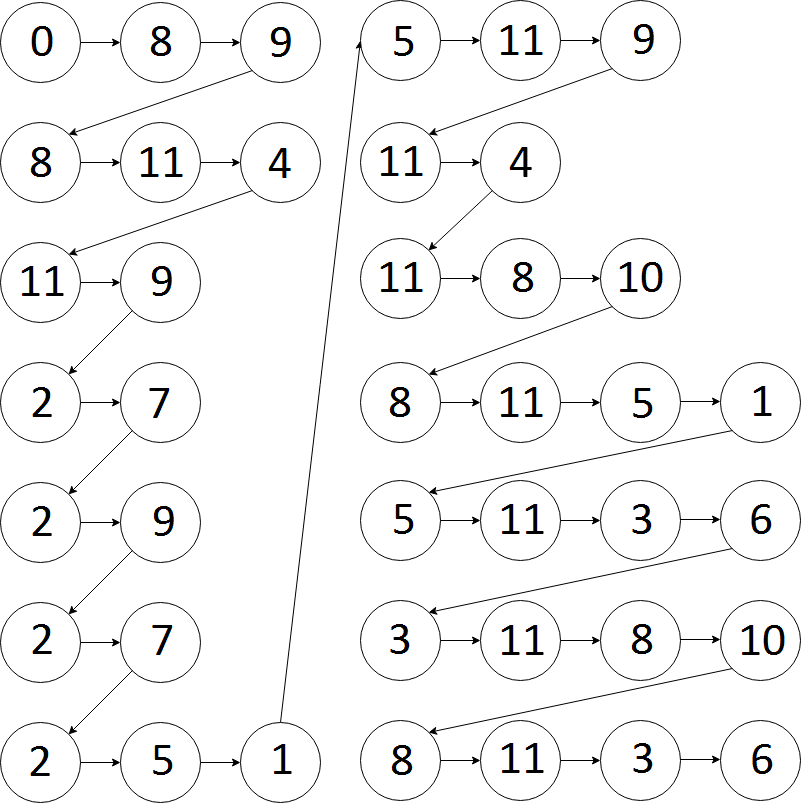
\includegraphics[width=0.5\textwidth]{img/img4.png}
  	\caption{The transportation solution path constructed by amalgamating supply and restock path segments}	
  	\label{fig:img4}
\end{figure}

Fig. \ref{fig:img4} demonstrates the solution path that the described algorithm suggests for a given instance of the problem acquired through the testing environment that produced the base graph with transportation problem parameters.


\section{Conclusion}
After observing the fundamenal operation principles of the proposed algorithm, it is important to note that such algorithm is capable of functioning with a wide spectrum of transportation problem instances. Under experimental conditions, the given algorithm launched on the demonstrated graph  with variable truck capacity produces economically useful and mathematically reasonable results. As seen from Table \ref{tab:tab1}, with increasing the truck capacity, the number of produced path segments and the cost of the overall path decreases.
 
\begin{table}[h]
\centering
\caption{Routing algorithm experimental results} 
\label{tab:tab1}
	\begin{tabular}{ | l | l | l |}
 		\hline
 		Truck Capacity & Number of path segments & Overall path cost \\ \hline
 		10 & 22 segments & 68360.5  \\ \hline
		15 & 16 segments & 48142.7 \\ \hline
		20 & 14 segments & 42781.1  \\ \hline
		22 & 13 segments & 40764.5 \\ \hline
		23 & 9 segments & 26577.2 \\ \hline
	\end{tabular}
\end{table}

However, it is notable that the change is not quite proportional. As seen on Fig. \ref{fig:img2} and Fig. \ref{fig:img3} below, changing the truck capacity produces a slope-like response in the cost reduction and in the number of path segments produced.

%\begin{figure}[h]
%\begin{tabular}{ll}
%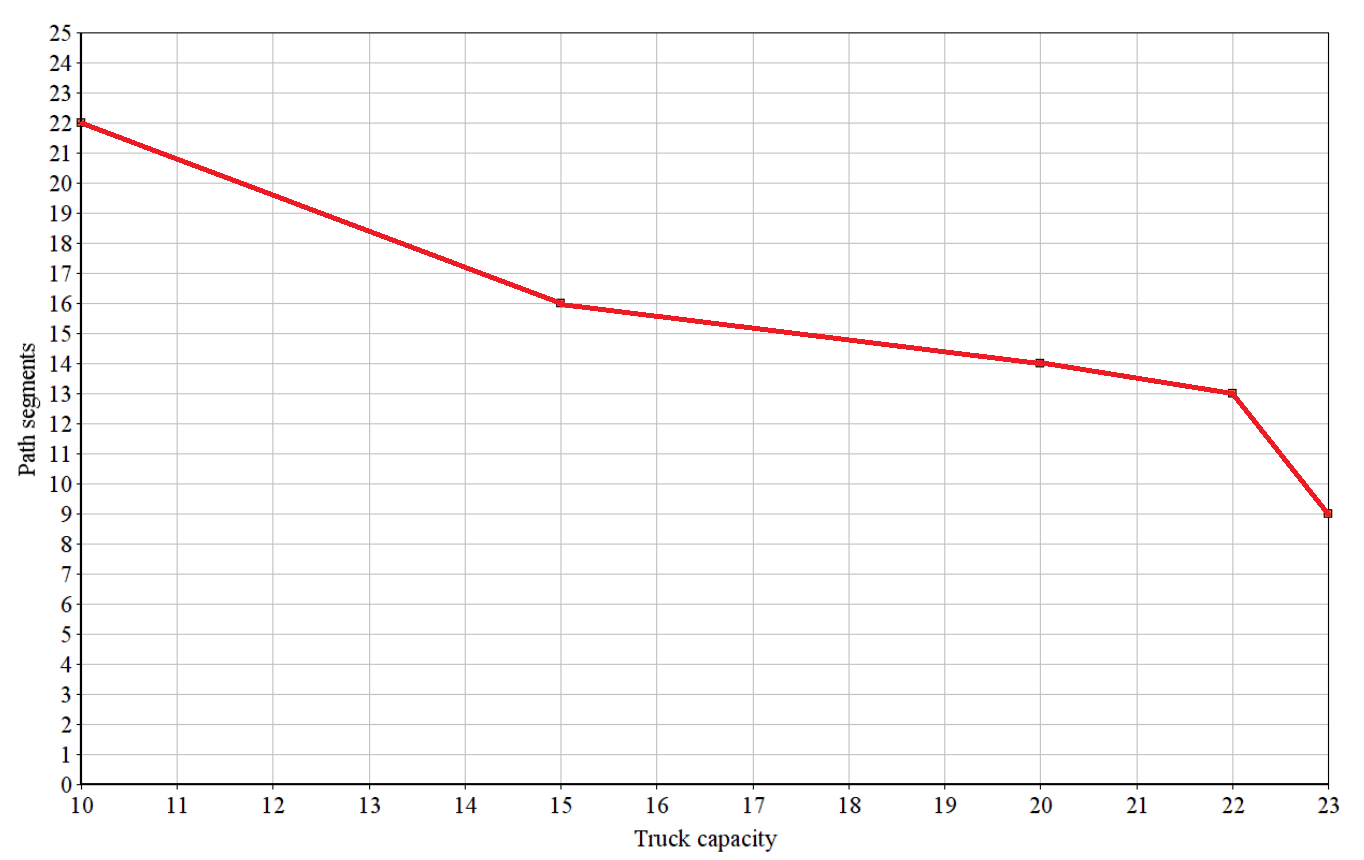
\includegraphics[width=0.5\textwidth]{img/img2.png}
%&
%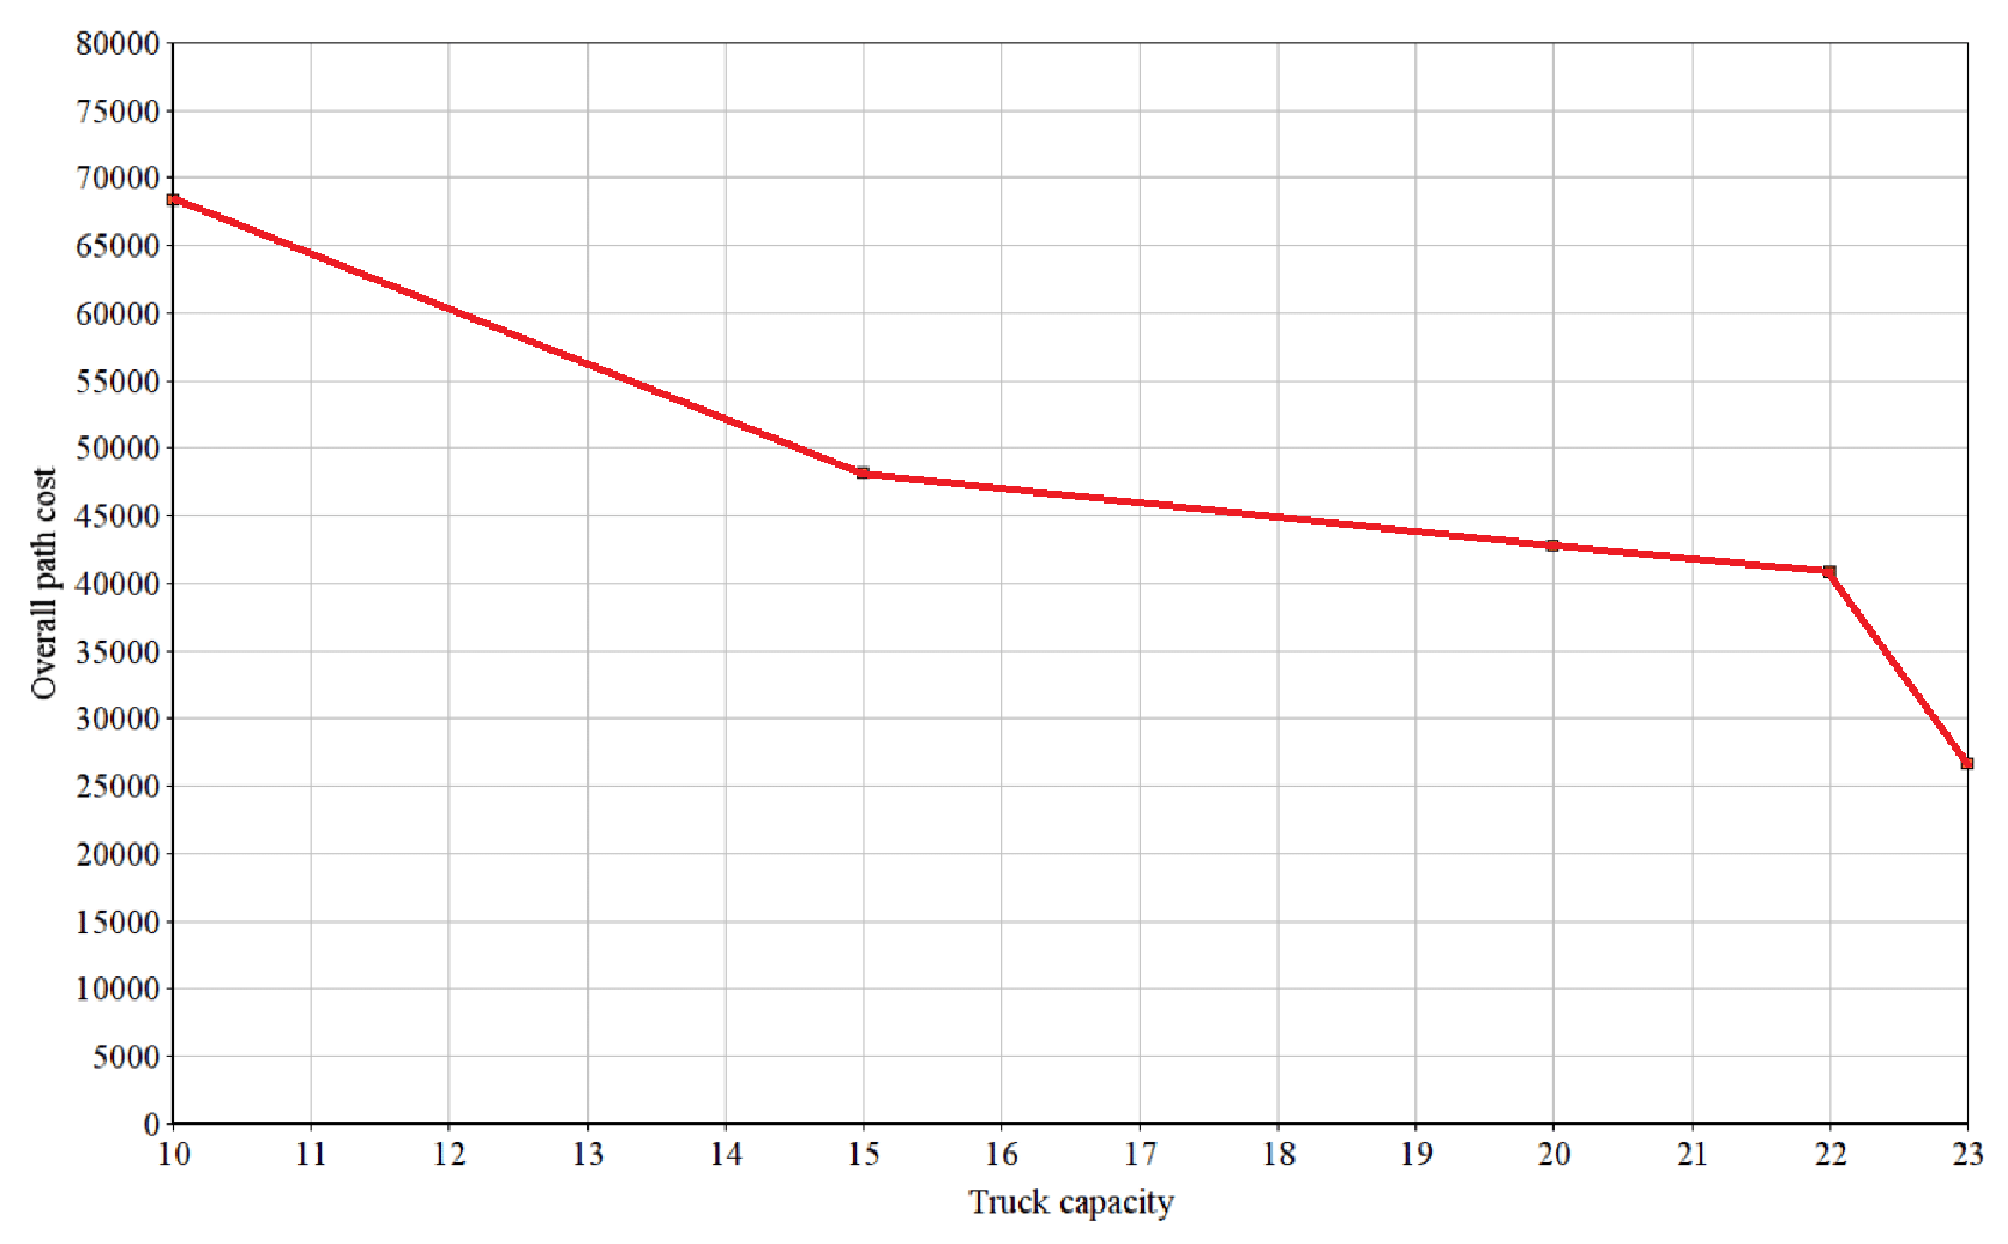
\includegraphics[width=0.5\textwidth]{img/img3.png}
%\end{tabular}
%\caption{Left: Truck capacity increase reduces the number of shipping path segments.
%Right: Truck capacity increase gradually reduces the overall path cost}
%\label{fig:img2}
%\end{figure}

\begin{figure}[h]
	\centering
  	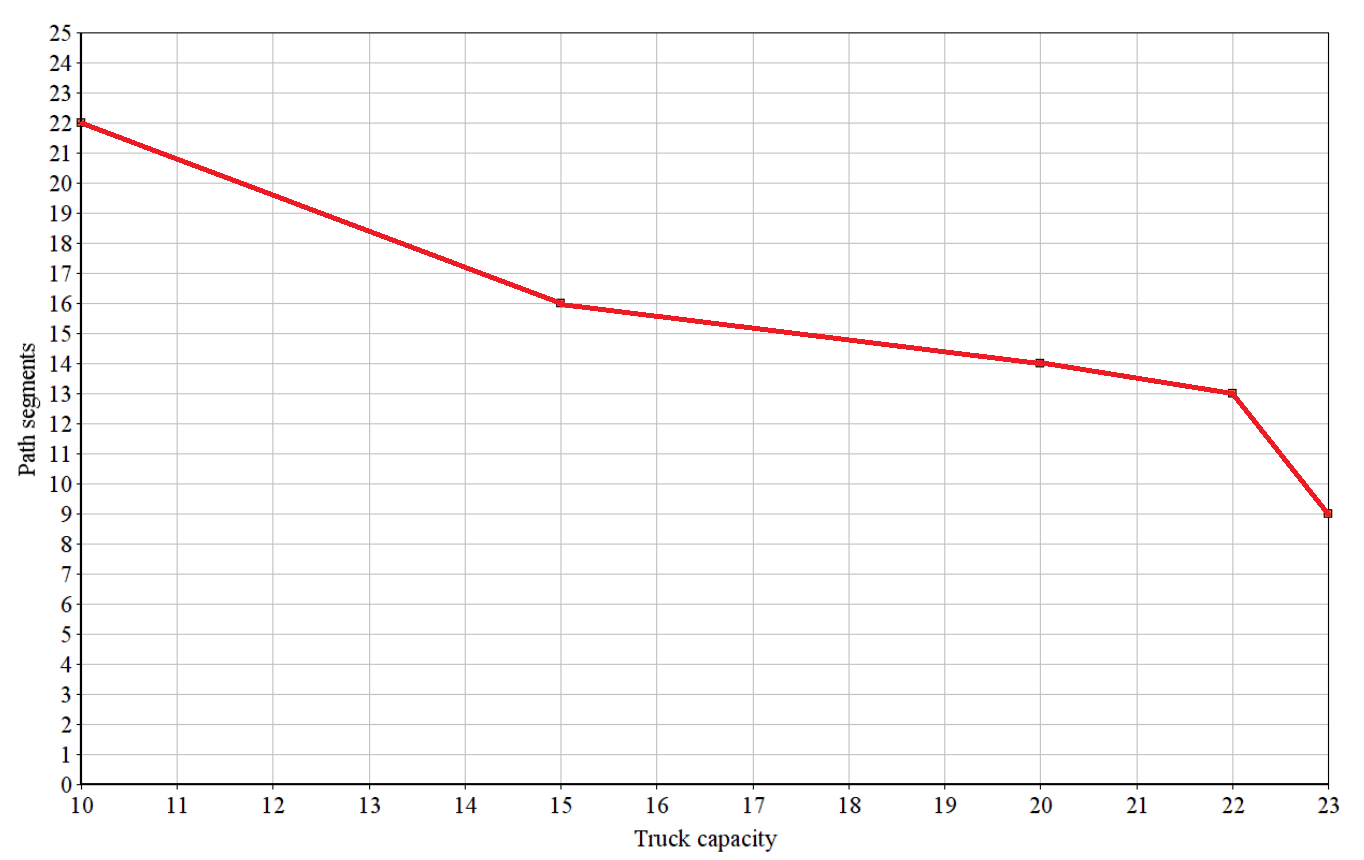
\includegraphics[width=0.6\textwidth]{img/img2.png}
  	\caption{Truck capacity increase reduces the number of shipping path segments}	
  	\label{fig:img2}
\end{figure}

\begin{figure}[h]
	\centering
  	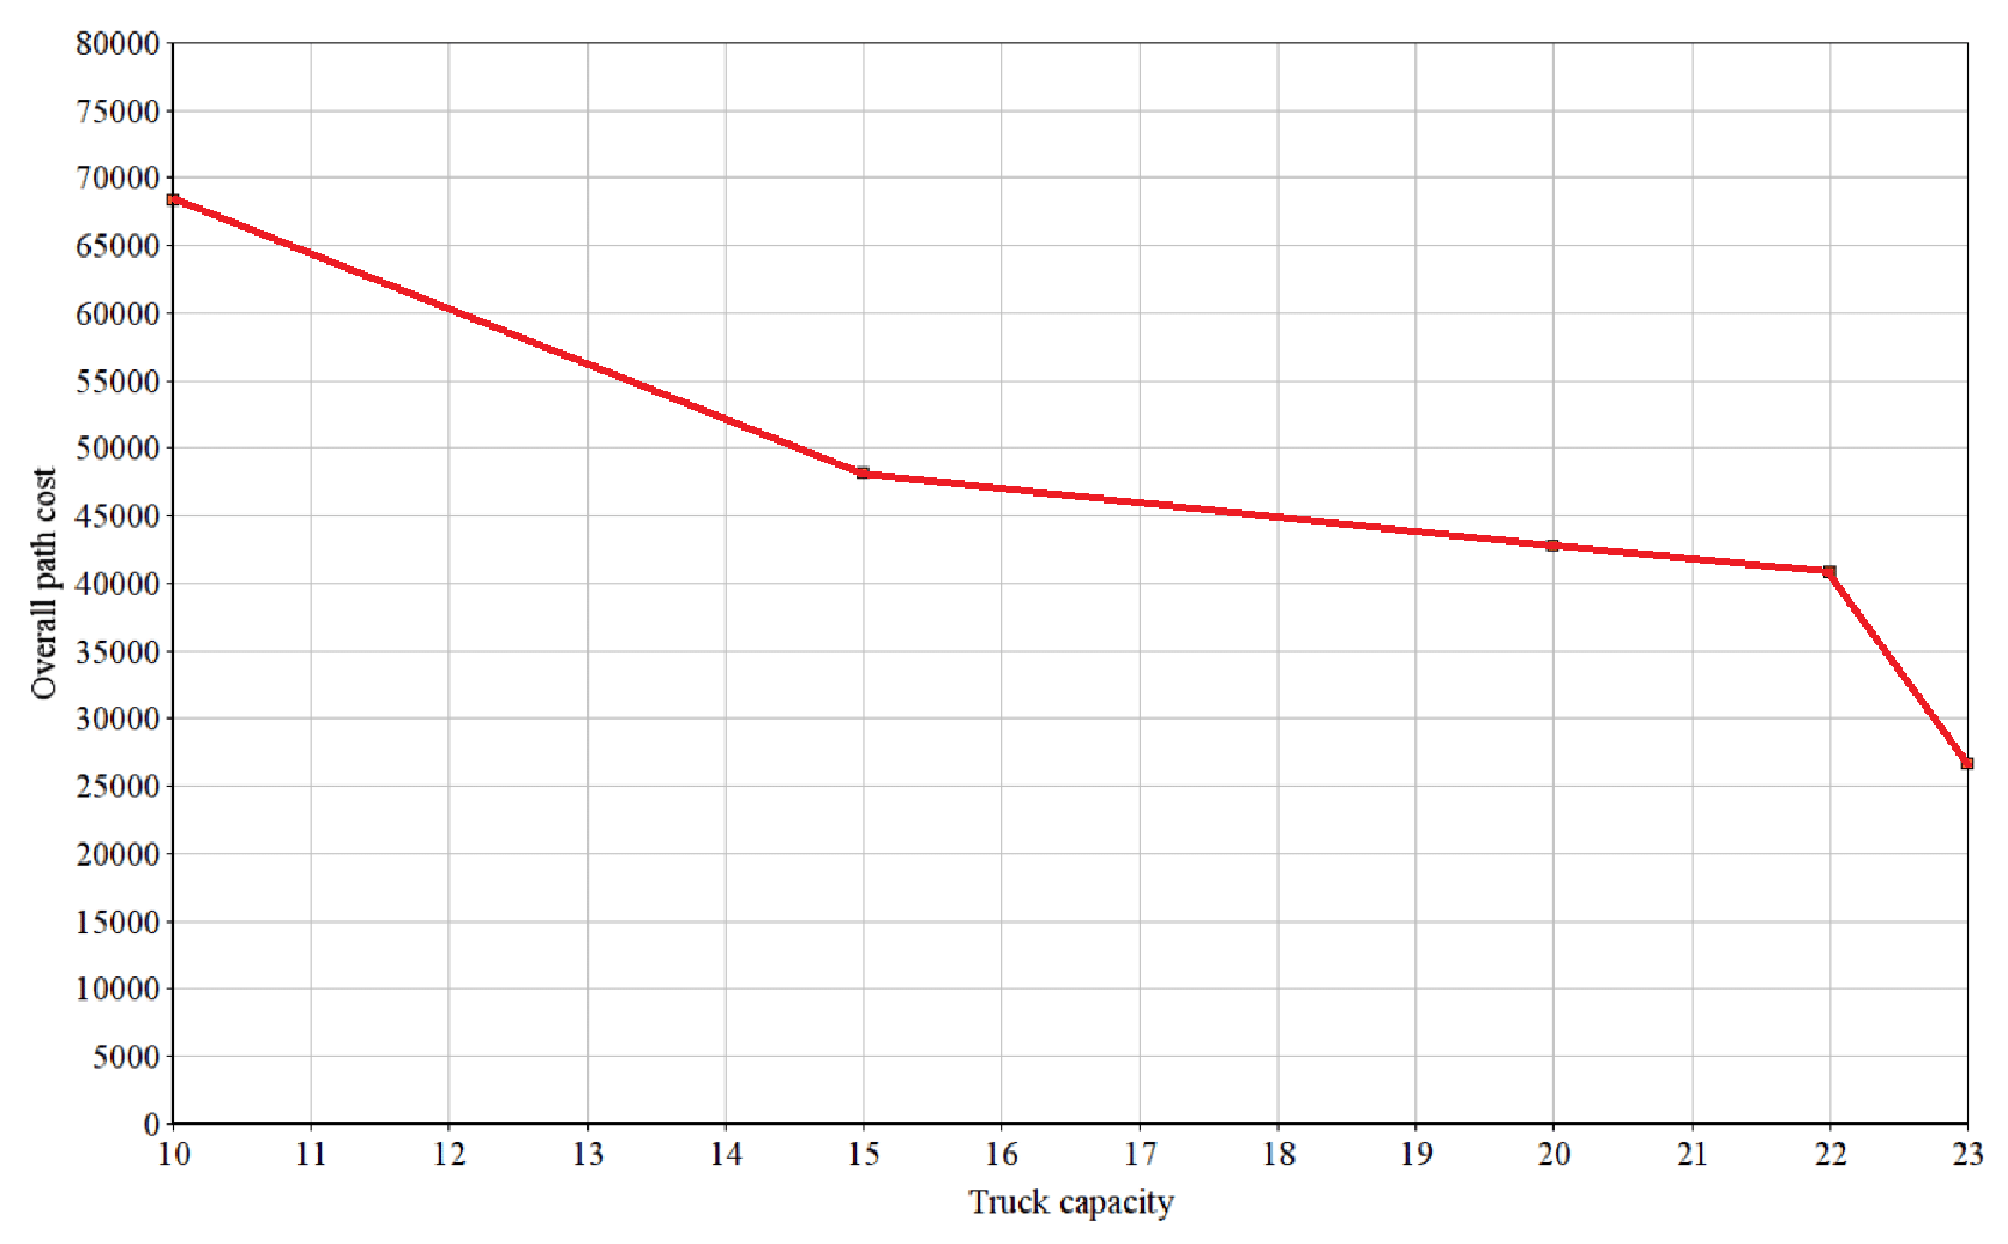
\includegraphics[width=0.6\textwidth]{img/img3.png}
  	\caption{Truck capacity increase gradually reduces the overall path cost}	
  	\label{fig:img3}
\end{figure}

Given such statistics, it is possible to estimate how much each added unit of capacity corresponds to the decrease in the overall solution cost for this particular instance of the problem. This directly translates into the economic reality of any business involving transportation of some items between certain locations on the map. Such algorithm is thus capable to provide not only a solution to the given problem with set parameters, but also \textit{an ability to estimate the potential alternatives to a given solution with different parameters}. 

What if one had to pick a bigger truck? How could extra expenses on deploying another truck be covered by saving on the number of trips between the map locations? What is the most efficient size of the truck, that can solve a given transportation problem on a given map? All these questions can eventually be answered by running the routing algorithm provided here several times with tweaked parameters. Basically, by solving the given problem with different parameters and combining the resulting data together, this algorithm can be used as a \textit{cost estimation tool}.

There are, however, major improvements potentially available to this algorithm. For example, the cost estimation function could involve more real-life factors affecting any transportation, such as: truck fuel consumption, desirability of paths (major city roads might not allow truck traffic coming through at certain times), required stops (drivers taking breaks and changing shifts) and more. Another improvement to deploy could be allowing multiple types of cargo, which considerably increases the complexity of decision-making and solving the transportation problem.

In the described algorithm, the decision-making heuristic of combined time and distance is only applied to selecting next place to go, so the overall cost is minimized per each segment of the solution path. However, sometimes the transportation problem can involve prioritizing time over cost, cost over time or other decision factor. Thus, wisely balancing the decision-making in the described routing algorithm along with dealing with various shipment types becomes the major design difficulty to overcome. 

The source code and related documentation with experimental data is located at the following GitHub repository:\\ 
\begin{center}
https://github.com/andreloboteixeira/cs820-project 
\end{center}







% needed in second column of first page if using \IEEEpubid
%\IEEEpubidadjcol

%\subsection{Subsection Heading Here}
%Subsection text here.

%\subsubsection{Subsubsection Heading Here}
%Subsubsection text here.

% An example of a floating figure using the graphicx package.
% Note that \label must occur AFTER (or within) \caption.
% For figures, \caption should occur after the \includegraphics.
% Note that IEEEtran v1.7 and later has special internal code that
% is designed to preserve the operation of \label within \caption
% even when the captionsoff option is in effect. However, because
% of issues like this, it may be the safest practice to put all your
% \label just after \caption rather than within \caption{}.
%
% Reminder: the "draftcls" or "draftclsnofoot", not "draft", class
% option should be used if it is desired that the figures are to be
% displayed while in draft mode.
%
%\begin{figure}[!t]
%\centering
%\includegraphics[width=2.5in]{myfigure}
% where an .eps filename suffix will be assumed under latex, 
% and a .pdf suffix will be assumed for pdflatex; or what has been declared
% via \DeclareGraphicsExtensions.
%\caption{Simulation results for the network.}
%\label{fig_sim}
%\end{figure}

% Note that the IEEE typically puts floats only at the top, even when this
% results in a large percentage of a column being occupied by floats.


% An example of a double column floating figure using two subfigures.
% (The subfig.sty package must be loaded for this to work.)
% The subfigure \label commands are set within each subfloat command,
% and the \label for the overall figure must come after \caption.
% \hfil is used as a separator to get equal spacing.
% Watch out that the combined width of all the subfigures on a 
% line do not exceed the text width or a line break will occur.
%
%\begin{figure*}[!t]
%\centering
%\subfloat[Case I]{\includegraphics[width=2.5in]{box}%
%\label{fig_first_case}}
%\hfil
%\subfloat[Case II]{\includegraphics[width=2.5in]{box}%
%\label{fig_second_case}}
%\caption{Simulation results for the network.}
%\label{fig_sim}
%\end{figure*}
%
% Note that often IEEE papers with subfigures do not employ subfigure
% captions (using the optional argument to \subfloat[]), but instead will
% reference/describe all of them (a), (b), etc., within the main caption.
% Be aware that for subfig.sty to generate the (a), (b), etc., subfigure
% labels, the optional argument to \subfloat must be present. If a
% subcaption is not desired, just leave its contents blank,
% e.g., \subfloat[].


% An example of a floating table. Note that, for IEEE style tables, the
% \caption command should come BEFORE the table and, given that table
% captions serve much like titles, are usually capitalized except for words
% such as a, an, and, as, at, but, by, for, in, nor, of, on, or, the, to
% and up, which are usually not capitalized unless they are the first or
% last word of the caption. Table text will default to \footnotesize as
% the IEEE normally uses this smaller font for tables.
% The \label must come after \caption as always.
%
%\begin{table}[!t]
%% increase table row spacing, adjust to taste
%\renewcommand{\arraystretch}{1.3}
% if using array.sty, it might be a good idea to tweak the value of
% \extrarowheight as needed to properly center the text within the cells
%\caption{An Example of a Table}
%\label{table_example}
%\centering
%% Some packages, such as MDW tools, offer better commands for making tables
%% than the plain LaTeX2e tabular which is used here.
%\begin{tabular}{|c||c|}
%\hline
%One & Two\\
%\hline
%Three & Four\\
%\hline
%\end{tabular}
%\end{table}


% Note that the IEEE does not put floats in the very first column
% - or typically anywhere on the first page for that matter. Also,
% in-text middle ("here") positioning is typically not used, but it
% is allowed and encouraged for Computer Society conferences (but
% not Computer Society journals). Most IEEE journals/conferences use
% top floats exclusively. 
% Note that, LaTeX2e, unlike IEEE journals/conferences, places
% footnotes above bottom floats. This can be corrected via the
% \fnbelowfloat command of the stfloats package.

% if have a single appendix:
%\appendix[Proof of the Zonklar Equations]
% or
%\appendix  % for no appendix heading
% do not use \section anymore after \appendix, only \section*
% is possibly needed

% use appendices with more than one appendix
% then use \section to start each appendix
% you must declare a \section before using any
% \subsection or using \label (\appendices by itself
% starts a section numbered zero.)
%


% you can choose not to have a title for an appendix
% if you want by leaving the argument blank



% Can use something like this to put references on a page
% by themselves when using endfloat and the captionsoff option.
\ifCLASSOPTIONcaptionsoff
  \newpage
\fi


\appendices

\section{Output listing}
\label{app1}
\lstset{basicstyle=\ttfamily}
\lstinputlisting[language=C,breaklines=true,caption={The output of the routing algorithm solving the problem},captionpos=b,showstringspaces=false,label=lst2]{output.txt}

% trigger a \newpage just before the given reference
% number - used to balance the columns on the last page
% adjust value as needed - may need to be readjusted if
% the document is modified later
%\IEEEtriggeratref{8}
% The "triggered" command can be changed if desired:
%\IEEEtriggercmd{\enlargethispage{-5in}}

% references section

% can use a bibliography generated by BibTeX as a .bbl file
% BibTeX documentation can be easily obtained at:
% http://mirror.ctan.org/biblio/bibtex/contrib/doc/
% The IEEEtran BibTeX style support page is at:
% http://www.michaelshell.org/tex/ieeetran/bibtex/
%\bibliographystyle{IEEEtran}
% argument is your BibTeX string definitions and bibliography database(s)
%\bibliography{IEEEabrv,../bib/paper}
%
% <OR> manually copy in the resultant .bbl file
% set second argument of \begin to the number of references
% (used to reserve space for the reference number labels box)
\begin{thebibliography}{1}

\bibitem{monge:monge}
G. Monge. \emph{Mémoire sur la théorie des déblais et des remblais. Histoire de l’Académie Royale des Sciences de Paris, avec les Mémoires de Mathématique et de Physique pour la même année}. , pages 666–704, 1781.

\bibitem{kanto:kanto}
L. Kantorovich. \emph{On the translocation of masses}. C.R. (Doklady) Acad. Sci. URSS (N.S.), 37:199–201, 1942.

\bibitem{web:web}
Graphviz.org. \emph{Graphviz - Graph Visualization Software}. 2019. [online] Available at: http://www.graphviz.org/ [Accessed 24 Mar. 2019].

\end{thebibliography}



%\vfill

% Can be used to pull up biographies so that the bottom of the last one
% is flush with the other column.
%\enlargethispage{-5in}



% that's all folks
\end{document}